%%%%%%%%%%%%%%%%%%%%%%%%%%%%%%%%%%%%%%%%%
% University/School Laboratory Report
% LaTeX Template
% Version 3.1 (25/3/14)
%
% This template has been downloaded from:
% http://www.LaTeXTemplates.com
%
% Original author:
% Linux and Unix Users Group at Virginia Tech Wiki 
% (https://vtluug.org/wiki/Example_LaTeX_chem_lab_report)
%
% License:
% CC BY-NC-SA 3.0 (http://creativecommons.org/licenses/by-nc-sa/3.0/)
%
%%%%%%%%%%%%%%%%%%%%%%%%%%%%%%%%%%%%%%%%%

%----------------------------------------------------------------------------------------
%	PACKAGES AND DOCUMENT CONFIGURATIONS
%----------------------------------------------------------------------------------------

\documentclass{article}

\usepackage[version=3]{mhchem} % Package for chemical equation typesetting
\usepackage{siunitx} % Provides the \SI{}{} and \si{} command for typesetting SI units
\usepackage{graphicx} % Required for the inclusion of images
\usepackage{natbib} % Required to change bibliography style to APA
\usepackage{amsmath} % Required for some math elements
\usepackage{tcolorbox} % Provide a frame around text
\usepackage{tabto}
\usepackage[normalem]{ulem}
\usepackage{listings}
\lstset{
  basicstyle=\ttfamily,
  columns=fullflexible,
  breaklines=true,
  postbreak=\mbox{\textcolor{red}{$\hookrightarrow$}\space},
}
\usepackage{geometry}
\geometry{
	left = 20mm,
	right = 20mm
}

\usepackage{french}

\setlength\parindent{0pt} % Removes all indentation from paragraphs

\renewcommand{\labelenumi}{\alph{enumi}.} % Make numbering in the enumerate environment by letter rather than number (e.g. section 6)

%\usepackage{times} % Uncomment to use the Times New Roman font

%----------------------------------------------------------------------------------------
%	DOCUMENT INFORMATION
%----------------------------------------------------------------------------------------

\title{Majeure info \\ TP - S\'{e}curit\'{e} Lab} % Title

\author{Nicolas \textsc{Lagaillardie}} % Author name

\date{\today} % Date for the report

\begin{document}

\maketitle % Insert the title, author and date

\tableofcontents
\newpage

%\begin{center}
%\begin{tabular}{l r}
%Date Performed: & January 1, 2012 \\ % Date the experiment was performed
%Partners: & James Smith \\ % Partner names
%& Mary Smith \\
%Instructor: & Professor Smith % Instructor/supervisor
%\end{tabular}
%\end{center}

% If you wish to include an abstract, uncomment the lines below
% \begin{abstract}
% Abstract text
% \end{abstract}

%----------------------------------------------------------------------------------------
%	SECTION 1
%----------------------------------------------------------------------------------------

\section{Objectif}

Le but du TP est de tester la s\'{e}curit\'{e} d'un serveur et d'exploiter ses diff\'{e}rentes failles de s\'{e}curit\'{e}. Nous utilisons pour cela une machine virutlle qui h\'{e}berge OpenSuse 11.2, et nous attaquerons le serveur depuis cette machine.
 
%----------------------------------------------------------------------------------------
%	SECTION 2
%----------------------------------------------------------------------------------------

\section{Analyse du traffic internet}

\paragraph{}
Voici les diff\'{e}rentes commandes utilis\'{e}es pour \'{e}tablir des connexions entre notre PC et la machine virtuelle \\*
\begin{tcolorbox}
\begin{lstlisting}[language=sh]
$ ifconfig
\end{lstlisting}
\begin{lstlisting}[language=sh]
$ netstat -an -t
\end{lstlisting}
\begin{lstlisting}[language=sh]
$ telnet [adresse ip]
\end{lstlisting}
\begin{lstlisting}[language=sh]
$ ftp [adresse ip]
\end{lstlisting}
\begin{lstlisting}[language=sh]
$ ssh [user]@[adresse ip]
\end{lstlisting}
\end{tcolorbox}
~\\*
\paragraph{}
Dans l'ordre, ces commandes permmettent de r\'{e}cup\'{e}rer l'adresse ip de la machine courante, de r\'{e}cup\'{e}rer le port TCP, et d'\'{e}tablir des une connections \textit{telnet} / \textit{FTP} / \textit{SSH} avec l'autre machine.

\paragraph{}
\textbf{Telnet} permet d'envoyer et recevoir des lignes de texte avec la machine distante. \\*
\textbf{FTP} permet d'envoyer et recevoir des fichiers. \\*
\textbf{SSH} permet d'ouvrir un terminal sur la machine distante, et donc d'en prendre le contrôle.
 
%----------------------------------------------------------------------------------------
%	SECTION 3
%----------------------------------------------------------------------------------------

\section{S\'{e}curit\'{e} de l'application}

\paragraph{}
Apr\`{e}s avoir d\'{e}marr\'{e} le serveur depuis notre machine, nous acc\'{e}dons \`{a} l'adresse \textbf{localhost:8080} sur la machine distante. Cela signifie que le port 8080 est maintenant occup\'{e} et indisponible pour tout autre type de connection. Voic une capture d'\'{e}cran de ce que nous obtenons :
\\*
\begin{figure}[h]
\begin{center}
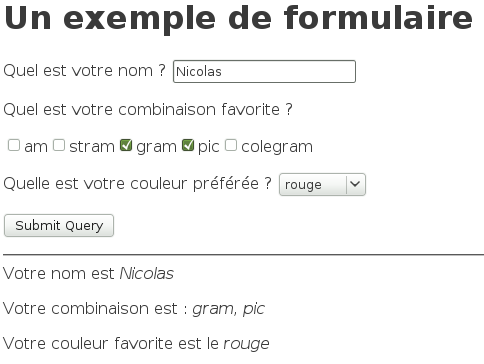
\includegraphics[width=0.64\textwidth]{second}
\caption{Screenshot de l'application}
\end{center}
\end{figure}
\newpage
%----------------------------------------------------------------------------------------
%	SECTION 4
%----------------------------------------------------------------------------------------

\section{Deny of service et buffer overflow}

\paragraph{}
Une premi\`{e}re attaque consiste \`{a} envoyer un nom bien trop lourd pour pouvoir \^{e}tre trait\'{e} correctement par le serveur. Cela r\'{e}sulte tout simplement en un crash du serveur, que l'on doit alors red\'{e}marrer. \\*
Une solution pour pr\'{e}venir cette attaque est de limiter la taille maximale de l'input et refuser l'input si la taille est trop importante. \\*
Une autre attaque consiste \`{a} simuler un tr\`{e}s grand nombre de connections simultan\'{e}es au serveur, un DDOS. Je n'ai pas pu le faire sur ma propre machine puisque c'est elle-m\^{e}me qui s'attaque (en terme d'hardware). Mais avec au moins deux machines distinctes, c'est possible. Dans ce cas, le serveur prend \'{e}norm\'{e}ment de temps pour r\'{e}pondre \`{a} une requ\^{e}te voir refuse toute requ\^{e}te et crash. Il n'existe pas de v\'{e}ritable solution \`{a} ce probl\`{e}me, et une alternative consiste \`{a} refuser des requ\^{e}tes provenant de ces requ\^{e}tes intempestives.

%----------------------------------------------------------------------------------------
%	SECTION 5
%----------------------------------------------------------------------------------------

\section{Ex\'{e}cution de commande \`{a} distance}

\paragraph{}
EN m'inspirant du code index.pl, voici un code un script bash qui demande quelques informations sur l'utilisateur et qui renvoie un \textbf{Bonjour [utilisateur]} ainsi que d'autres informations sur la machine de l'utilisateur. \\*
\begin{tcolorbox}
\begin{lstlisting}[language=sh]
#!/bin/bash
echo "Content-type: text/html"
echo ""
echo "<html><head><title>Bash as CGI"
echo "</title></head><body>"

echo "<h1>General system information for host $(hostname -s)</h1>"
echo ""

echo "<h1>Memory Info</h1>"
echo "<pre> $(free -m) </pre>"

echo "<h1>Disk Info:</h1>"
echo "<pre> $(df -h) </pre>"

echo "<h1>Logged in user</h1>"
echo "<pre> $(w) </pre>"

echo "<center>Information generated on $(date)</center>"
echo "</body></html>"

echo Bonjour $FORM_civilite $FORM_prenom $FORM_nom <!-- affichage de la civilit\'{e}, du prenom et du nom de la personne -->

cat << EOF
</h2>
</center>
<hr>
</body>
</html>
EOF
\end{lstlisting}
\end{tcolorbox}
~\\*
\paragraph{}
Pour corriger ce "d\'{e}faut", il faut d\'{e}sactiver les scripts CGI sur le serveur, ce qui peut se faire \`{a} l'aide de cette commande.\\*
\begin{tcolorbox}
\begin{lstlisting}[language=sh]
$ a2dismod cgi
\end{lstlisting}
\end{tcolorbox}

%----------------------------------------------------------------------------------------
%	SECTION 6
%----------------------------------------------------------------------------------------

\section{Cross site scripting}

\paragraph{}
Pour exploiter des failles concernant les messages d'erreur renvoy\'{e}s par le serveur, nous avons inject\'{e} du code Javascript directement dans l'input. Le code suivant permet par exemple de connaître directement la valeur des cookies de la session actuelle.\\*
\begin{tcolorbox}
\begin{lstlisting}[language=html]
<script>
	alert(document.cookie)
</script>
\end{lstlisting}
\end{tcolorbox}

\end{document}